\chapter{The International Forest Monastery}

In January 1976, Wat Pah Nanachat was made up of one grass roof
\emph{sala} with a dirt floor, and a collection of a few very simple
kutis. Upon entering the monastery, my first impression was one of
seeing Tan Pabakharo, the tall, American monk I had met outside the
temple at Wat Boworn, sitting cross-legged on a bamboo platform doing
crochet. I don't know what I had expected but it was not that.

Once again, it appears my memory of arriving at places is consistently
vague, however I do still have an overall impression of how it felt to
be there for those few days. To me the atmosphere was a combination of
focused spiritual aspiration, pioneering spirit, and New Age adventure.
Ajahn Sumedho's confidence and joy were infectious. Although the group
of mostly Western monks and novices living there all appeared to be
strong-headed individuals -- there were no sycophants -- the quality of
Ajahn Sumedho's commitment and understanding was what fuelled the
community. There was a sense of `we are all in this together', but his
leadership was genuinely respected. The monastery followed more or less
the same routine as Wat Pah Pong: morning and evening puja, daily
alms-round, water hauling, leaf sweeping and robe making. Thankfully
though, there was none of the heaviness I had experienced at Wat Pah
Pong. In fact there was a lightness, a kindness, a quality of willing
cooperation.

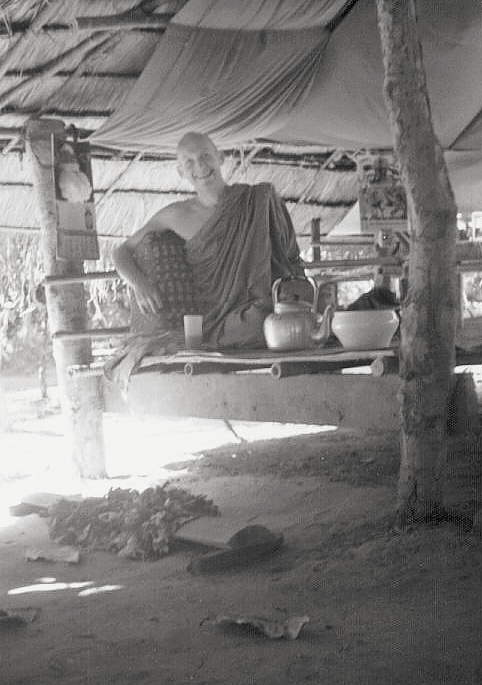
\includegraphics[width=3.21319in,height=4.56667in]{media/image2.jpeg}

It didn't take long before I was feeling that I could fit in there. The
community made me feel welcome, and gladly, the fact that technically I
belonged to the Dhammayutta sect didn't seem to make any difference: I
was treated as any other monk would be treated. Since nearly everyone
other than Ajahn Sumedho was relatively junior in the training, my place
in the line was fairly near the top, near where Tan Jotiko was sitting.

Jutta was staying with generous supporters of the monastery about
fifteen kilometres away in the town of Ubon, and would come out to visit
us during the day. As I have mentioned earlier, I was pleased that she
could meet Tan Ajahn Chah and had a chance to taste the authenticity of
this tradition and these teachings. The photo above of Ajahn Sumedho in
the grass roofed \emph{sala} was taken by Jutta.

There seemed to be no question about my being welcome to join the
community at Wat Pah Nanachat, but there was a question about the
correct way to handle the issue of the two different sects. It was
decided that I would have to go over to Wat Pah Pong and see what Tan
Ajahn Chah had to say about it.

Probably Tan Varapañño accompanied me, as he was considered one of the
most skilled in translating. Tan Ajahn Chah was very straightforward
about the matter: `Whatever your \emph{Upaccaya} (Preceptor), Tan Somdet
Nyanasamvara says, simply move here to live in this community, or
disrobe and formally request acceptance (\emph{Upasampada}) anew'. He
made it clear I was welcome regardless. You might think I would recall
my first meeting with Tan Ajahn Chah, but I don't, other than that
exchange about merely practical matters.

I suspect for the first time in many months I was beginning to feel
somewhat positive. `Yes, this is doable, and not just doable -- it is
genuinely desirable.' I could say with confidence that I really wanted
to live in this place and practise with these people. Thank you, Ajahn
Sumedho and the sangha of Wat Pah Nanachat in 1976.

Jutta and I returned to Bangkok and I began the process of taking leave
from Phra Somdet and Wat Boworn. Josie Stanton helpfully arranged some
white clothes for me. The plan was that I would stay in Bangkok so long
as Jutta was there and then return to Wat Pah Nanachat. Jutta was
staying in a modest hotel on Khao San road which was near Wat Boworn,
close to where I would walk in the morning on alms-round.

The actual disrobing was difficult. Phra Somdet was gracious and
generous as ever, and made it clear that all he was concerned about was
my being contented living the Buddhist monk's life; and whenever I came
to Bangkok I was always welcome to stay at Wat Boworn (which I did until
I left Thailand in 1979.) I cried as I bowed in front of him; disrobing
was not what I wanted to be doing, but I could accept that it was an
expedient means to an end. If Thai monastic culture required that I go
through this process, then that was OK, even though it was painful.

To suddenly be walking around on the streets of Bangkok as a layman,
when inwardly I still felt myself to be committed to the life of a monk,
was weird. In retrospect, I see it taught me something valuable about
how the robes do not truly define who I am. They are a convention -- a
valuable one, but in reality they do not change who or what I am. In the
Dhammapada, verse 9, the Buddha says:

\emph{Wearing the robe of a renunciate\\
does not in itself render one pure.\\
Those who wear it and yet lack diligence\\
are heedless.}

When I returned to Wat Pah Nanachat, wearing white, I was given a seat
out the back of the \emph{sala}, almost at the bottom of the line. An
American psychiatrist, Gary was there, as was Bruce, an Australian I had
met some months earlier in Bangkok. I thought he had been headed for
Japan, but while he was in Nong Khai on a meditation retreat, his guitar
had been stolen and apparently that contributed to his giving up his
travels and deciding to take up monastic training under Ajahn Sumedho.
Also during that brief period when I was back down in Bangkok, Tan
Tiradhammo had arrived to join the community. He was a particularly
affable Canadian monk who had previously lived at Wat Umong in
Chiangmai.

The simplicity and modesty of the life was enjoyable, as was the
companionship. We each had our own kuti so there was plenty of private
time, but there were also regular periods of group practice and group
work. Sweeping leaves and pulling water from the well happened daily, as
did morning alms-around and pujas. From time to time we would meet up to
wash and dye robes, which was a hot and sweaty process. Bathing took
place at a communal area where a few square metres of the otherwise
dense undergrowth had been cleared and half a dozen large clay water
jars had been set up. For shaving, there was a very small mirror sitting
on a makeshift shelf, or perhaps it was wedged into a cleft in a tree.

When I met Tan Ajahn Chah again, he commented that maybe I would have to
wait something like five years before taking my monk's robes again; but
he wasn't being serious. His ability to jest without being frivolous or
unkind was endearing. Just as a chiropractor might massage the client
before performing a manipulation, Tan Ajahn Chah had ways of putting
people at ease, making them pliable, before delivering not so
easy-to-receive teachings.

I think it was around May or June that year that Gary, Bruce and I were
called over to Wat Pah Pong to prepare for the \emph{Upasampada}. We had
already sewn our robes and presumably had a good grasp of the chanting;
now we would just wait until we got the word that Tan Ajahn Chah was
ready to perform the Precept Ceremony. At Wat Pah Pong we met an English
chap called Alan who was also preparing to take Precepts. He and I had
met at Wat Boworn where he had explained to me that he had been a monk
before with Tan Ajahn Chah but had left; now he was ready to rejoin.

This period coincided with Tan Ajahn Chah having a massive
\emph{Uposatha} temple constructed right in the centre of the monastery.
He let it be known that he wanted the temple built on top of a hill, and
for it to have open sides so a cool breeze could blow through. An extra
advantage of building it that way was that there would be space in the
foundations for large water storage tanks. The main issue, however, was
that there was no hill. Accordingly, a large lake was excavated outside
the walls of the main monastery of Wat Pah Pong; the soil which was
removed was then trucked inside the monastery to the site of the temple
building. Three or four metre high concrete retaining walls had already
been built, so that when the trucks dumped the soil, there was the task
of somehow getting it over the walls, spreading it out and pounding it.
All the monks and novices and nuns that were available joined in.
Initially the nuns (\emph{maechee}) were outside, throwing the soil over
the walls, and we were on the inside collecting it, spreading it, and
pounding it. Then we swapped places. It was solid, hard work which began
soon after the morning meal at 8 am and continued right through the day
until late in the evening, sometimes until midnight. Thankfully, the 3
am morning pujas had been temporarily suspended. To help keep us fit and
healthy, senior monks would walk down the line at the mealtime handing
out vitamin pills.

On the evening of 21st June 1976, as we were making our way back to our
kutis after water hauling, Tan Ajahn Chah made a gesture that indicated
we should get ready. None of the four of us -- Gary, Bruce, Alan or
myself -- must have really understood what he meant, because we were
comfortably sitting round chatting, having a jolly brew-up, when someone
appeared asking if we could make our way over to the \emph{sala} since
the sangha, including Ajahn Sumedho who had come over from Wat Pah
Nanachat, were waiting. How did that happen? This was worse than my
towering over Phra Somdet telling him that I wanted him to accept me as
a Samanera.

Needless to say, we quickly gathered our wits and our robes and made our
way over to the \emph{sala}. Indeed, the entire assembly of the Wat Pah
Pong sangha was waiting for us. The ceremony began with our being
formally offered our robes and bowl; in my case it was by the parents of
Tan Pabakharo, who were visiting at the time. The chanting
\emph{acariyas} for Gary and myself were Ajahn Liem (later to become
abbot of Wat Pah Pong) and Ajahn Sawaeng. My new name was Uppanno
Bhikkhu. What an extraordinary privilege. I am profoundly indebted and
grateful to Tan Ajahn Chah and the sangha at Wat Pah Pong.

